\documentclass{beamer}

\usetheme{Madrid}

\mode<presentation>
{ \usetheme{boxes} }

\usefonttheme[stillsansseriftext]{serif}
%\usepackage{times}  % fonts are up to you
\usepackage{graphicx}
\usepackage{natbib}
\usepackage{amsmath}

\setbeamercovered{transparent}


\setbeamertemplate{footline}[text line]{%
  \parbox{\linewidth}{\hfill\insertshortauthor\hfill\insertpagenumber}}
\setbeamertemplate{navigation symbols}{}


\AtBeginSection[]
{
  \begin{frame}
    \frametitle{Outline}
    \tableofcontents[currentsection]
  \end{frame}
}


%%%%%%%%%%%%%%%%%%%%%%%


\bibliographystyle{aa_anja}

\citestyle{aa}
\bibpunct{(}{)}{;}{a}{}{,}

\def\aj{AJ}%
          % Astronomical Journal
\def\araa{ARA\&A}%
          % Annual Review of Astron and Astrophys
\def\apj{ApJ}%
          % Astrophysical Journal
\def\apjl{ApJ}%
          % Astrophysical Journal, Letters
\def\apjs{ApJS}%
          % Astrophysical Journal, Supplement
\def\aap{A\&A}%
          % Astronomy and Astrophysics
\def\aapr{A\&A~Rev.}%
          % Astronomy and Astrophysics Reviews
\def\aaps{A\&AS}%
          % Astronomy and Astrophysics, Supplement
\def\mnras{MNRAS}%
          % Monthly Notices of the RAS
\def\nat{Nature}%
% Nature
\def\pasp{PASP}%
          % Publications of the ASP
\def\pasj{PASJ}
\def\physrep{Phys.~Rep.}%
          % Physics Reports
\let\apjlett=\apjl

\def\newblock{}

%%%%%%%%%%%%%%%%%%%%%%%%%%%%%%%%%%

%% these will be used later in the title page
%\title{Weighing the Giants}
%\subtitle{Calibrating X-ray Hydrostatic-Equilibrium Masses \\
%w/ Accurate Weak Lensing}
%\author[Applegate]{Douglas Applegate}
%\institute{%Argelander Institut f\"ur Astronomie \\
%\includegraphics[width=0.2\textwidth]{../figures/unilogo}\quad\includegraphics[width=0.2\textwidth]{../figures/aifa_logo}\\
%%Rheinische Friedrich-Wilhelms-Universit\"at Bonn \\ 
%with:\\
%{\scriptsize \textbf{Lensing:} Anja von der Linden (DARK), Patrick Kelly (Berkeley), Mark Allen, \\Dave Burke (KIPAC), Pat Burchat (KIPAC), Harald Ebeling (Hawaii)}\\
%{\scriptsize \textbf{X-ray:} Adam Mantz (Chicago), Steve Allen (KIPAC), Glenn Morris (KIPAC), \\David Rapetti (DARK), Robert Schmidt (Heidelberg)}
%}
%\date{1 July 2013 : Sesto}


%%%%%%%%%%%%%%%%%%%%%%%%%%%%%%%%%%%%


\begin{document}

%%%%%%%%%%%%%%%%%%%%%%%%%%%%%%%%%%%%%

%% this prints title, author etc. info from above
%\begin{frame}
%\titlepage
%\end{frame}
%
%%%%%%%%%%%%%%%%%%%%%%%%%%%%%%%%%%%%%%




\begin{frame}
\frametitle{The Situation at last report}

\centering

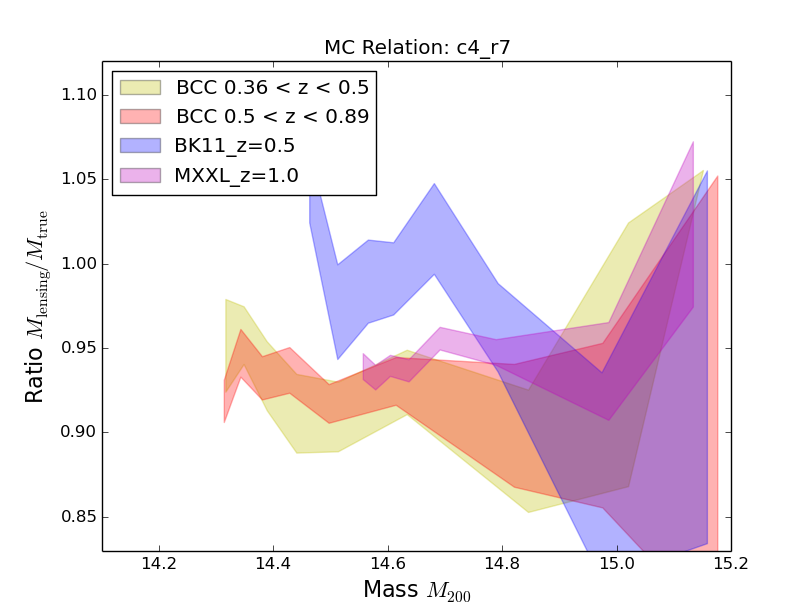
\includegraphics[width=0.45\textwidth]{../figures/c4_r7}
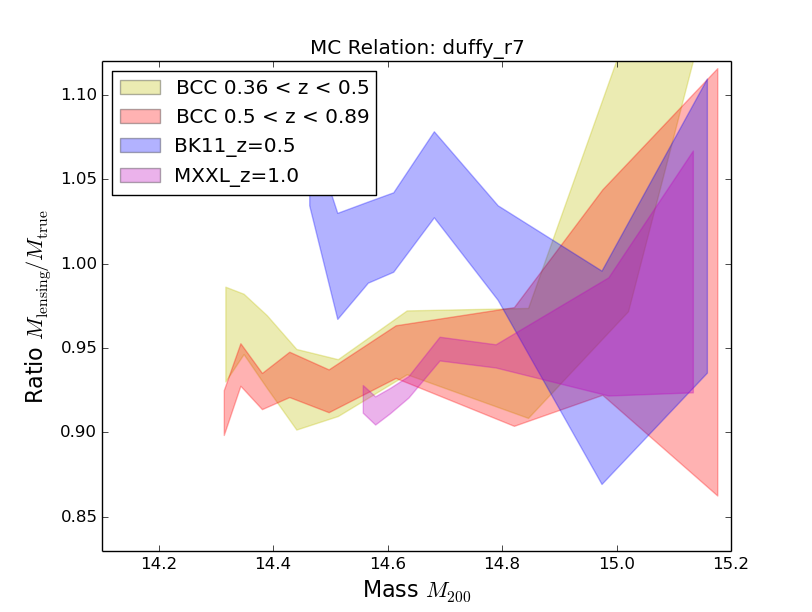
\includegraphics[width=0.45\textwidth]{../figures/duffy_r7}

{\small Plot of bias versus mass. Left: Assuming c=4, Right: Assuming Duffy08. The fit range is 0.5 - 3.0 Mpc. The width of each colored band represents the $1\sigma$ uncertainty in the median bias for each mass bin.}





\end{frame}

%%%%%%%%%%%%%%%%%%%%%%%%%%%%%%%%%%%%%%%

\begin{frame}
\frametitle{M-C Cosmology Dependence}
\centering

\includegraphics[height=0.9\textheight]{ludlow13mc.jpg}

\vspace{-25pt}

{\tiny M-C cosmology dependence, from Ludlow et al.\ 2013.}


\end{frame}

%%%%%%%%%%%%%%%%%%%%%%%%%%%%%%%%%%%%%%%

\begin{frame}
\centering

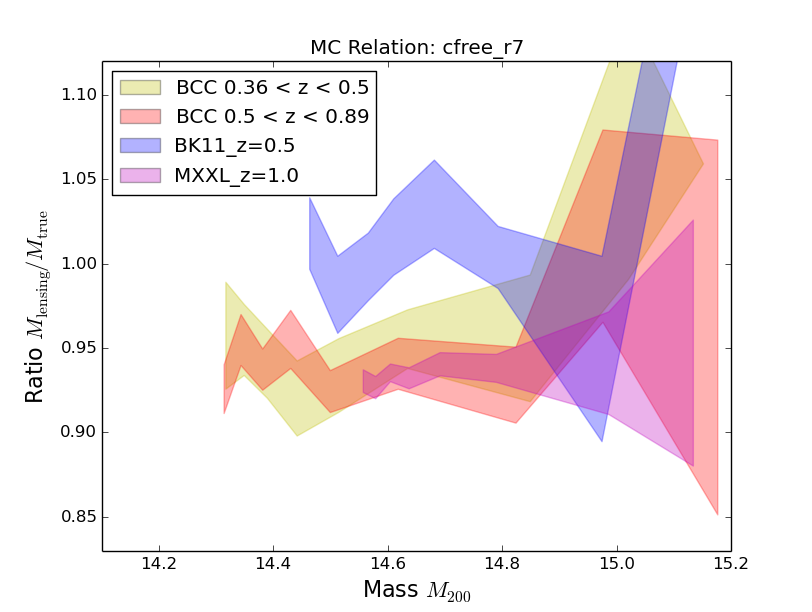
\includegraphics[width=0.65\textwidth]{../figures/cfree_r7}

{\small
Working on: Cosmology-dependent M-C relation (Zhao et al.\ 2008)\\
Question: Why is BK11 different?\\
Question: Are there other hidden cosmology dependencies (eg, substructure)?
}

\end{frame}

%%%%%%%%%%%%%%%%%%%%%%%%%%%%%%%%%%%%%

\begin{frame}

\centering

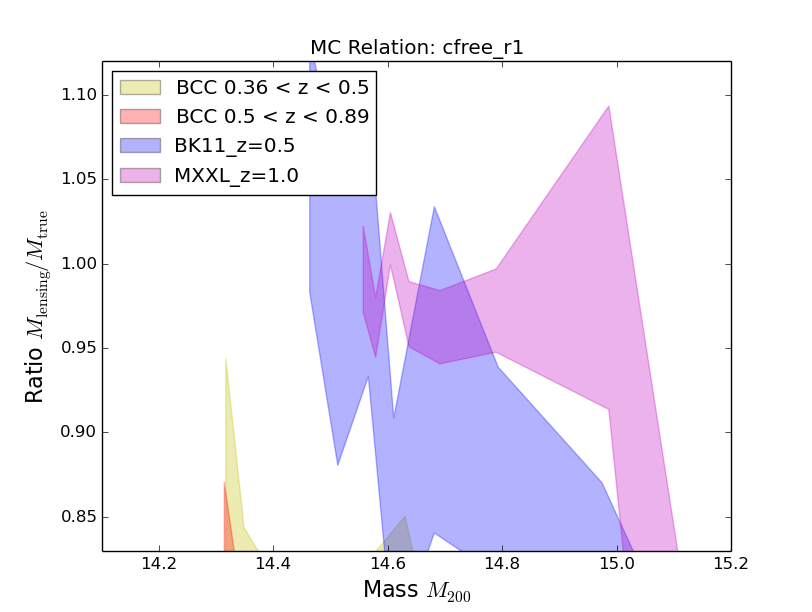
\includegraphics[width=0.65\textwidth]{../figures/cfree_r1}

\small{
C-free. 0.25 - 0.5 Mpc. \\


Problem at the cluster core? No...
}

\end{frame}

%%%%%%%%%%%%%%%%%%%%%%%%%%%%%%%%%%%%%%

\begin{frame}

\frametitle{Controlling for Noise Levels}
\centering

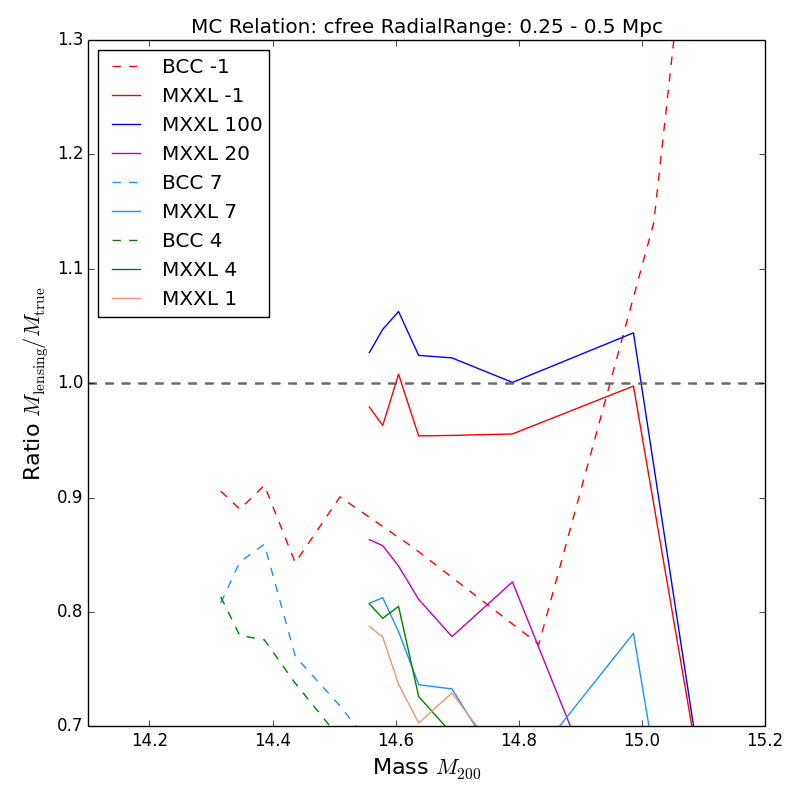
\includegraphics[width=0.45\textwidth]{../figures/density_cfree-r1}
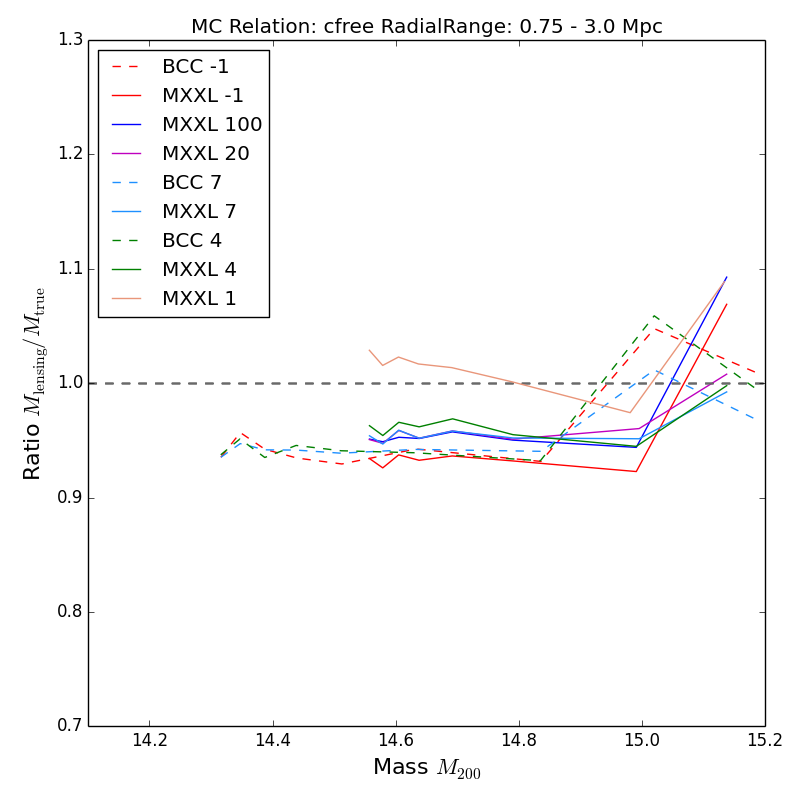
\includegraphics[width=0.45\textwidth]{../figures/density_cfree-r10}\\
\tiny{
Bias measured from the BCC and MXXL simulations. No shape noise is added, but different sampling densities are used. Left, right are different fit radii.
}

\small{
Subtle, but possibly different reactions to changing noise levels.
}
\end{frame}

%%%%%%%%%%%%%%%%%%%%%%%%%%%%%%%%%%%%%%

\begin{frame}
\frametitle{Effect of Noise}
\centering

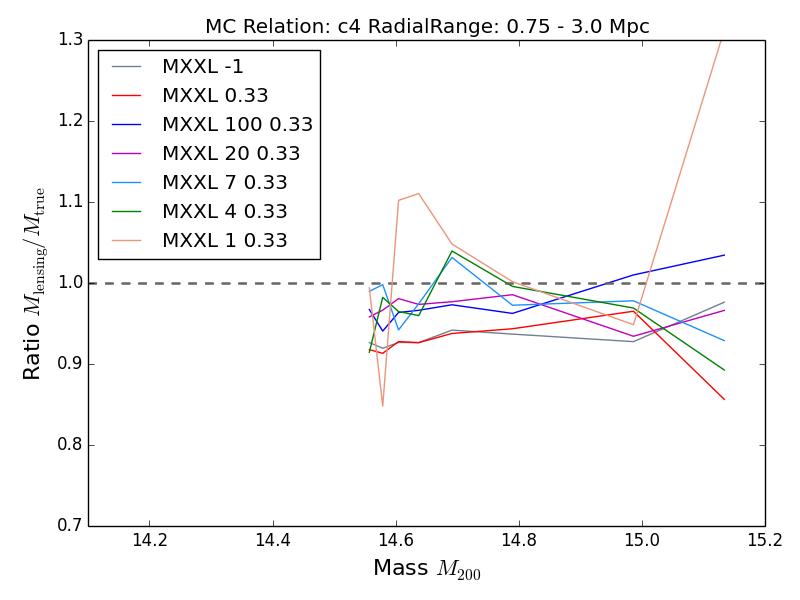
\includegraphics[width=0.45\textwidth]{../figures/density_noise2_c4-r10.png}
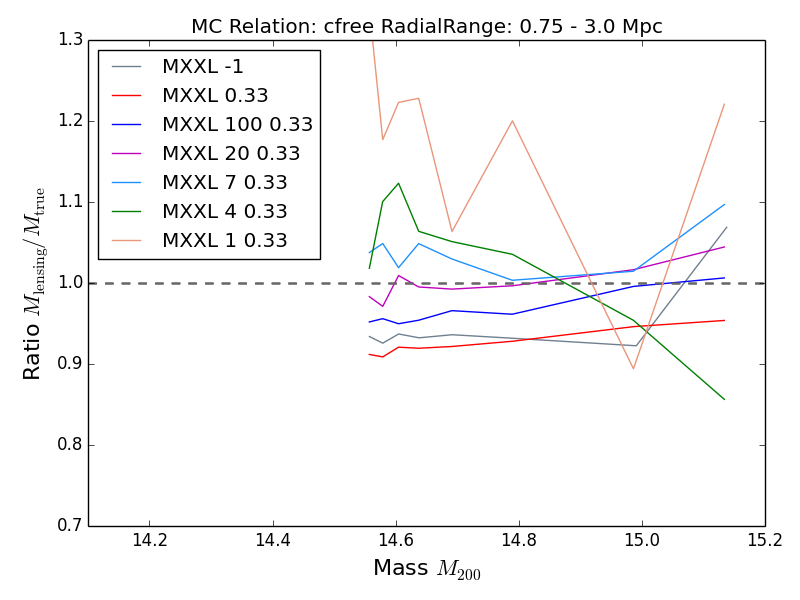
\includegraphics[width=0.45\textwidth]{../figures/density_noise2_cfree-r10}\\
{\tiny Shape noise + changing sample density. Left: M-C fixed, Right: C-free.}

{\small
Is this just noise bias, and can we properly account for it?
}

\end{frame}

%%%%%%%%%%%%%%%%%%%%%%%%%%%%%%%%%%%%%%%%

\begin{frame}
\frametitle{Why are intrinsic noise levels different?}

\centering

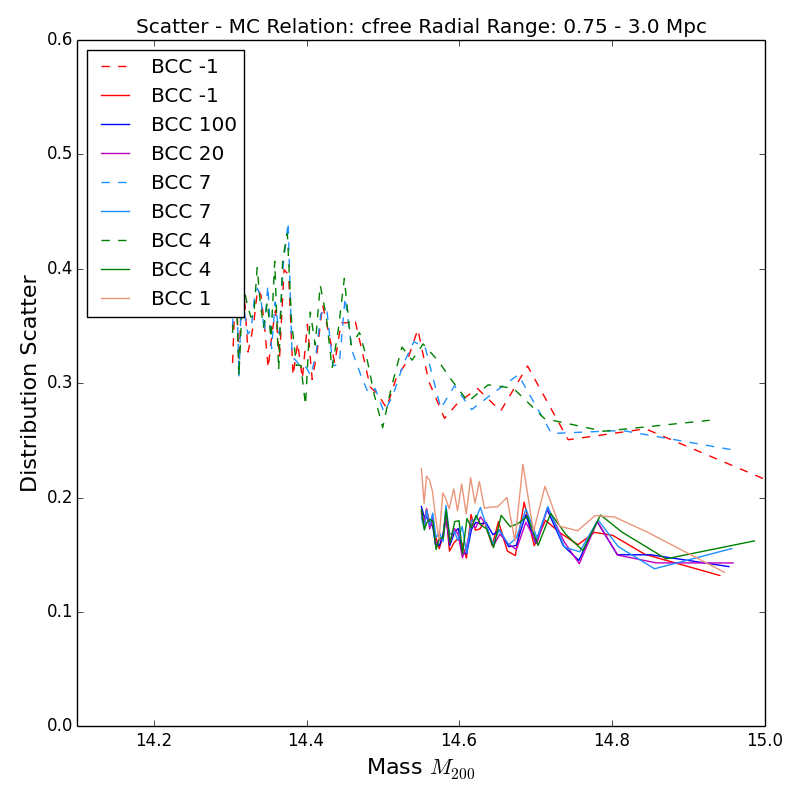
\includegraphics[height=0.65\textheight]{../figures/density_cfree-r10_scatter}\\
\tiny{Scatter from BCC and MXXL, under a range of sampling densities. Solid is MXXL, dotted is BCC. }


\small{BCC has much higher intrinsic noise. Is this light cone vs 200Mpc box? (Probably)}

\end{frame}

%%%%%%%%%%%%%%%%%%%%%%%%%%%%%%%%%%%%%%%

\begin{frame}
\frametitle{Realistic Shape Noise Dominates}

\centering

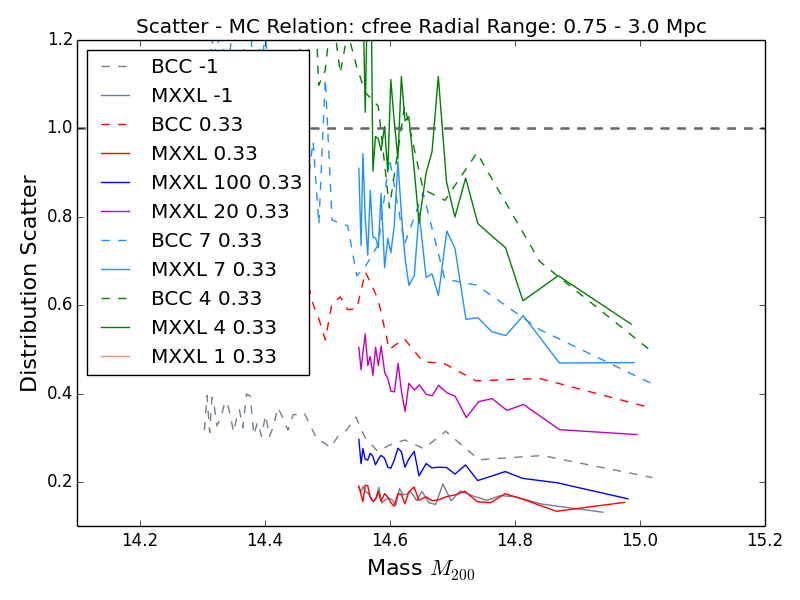
\includegraphics[width=0.65\textwidth]{../figures/density_noise2_cfree-r10_scatter}\\

{\tiny Scatter measured in BCC \& MXXL w/ shape noise + finite sampling.}


\end{frame}

%%%%%%%%%%%%%%%%%%%%%%%%%%%%%%%%%%%%%%

\begin{frame}
\frametitle{Redshift Bias Evolution}

\centering

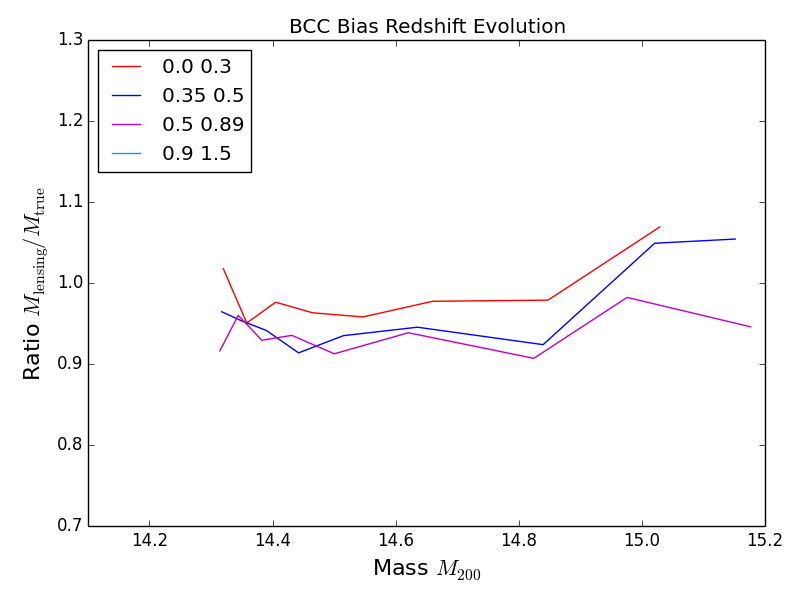
\includegraphics[width=0.65\textwidth]{../figures/bcc_bias_redshift_evo_r10_n0_0}\\
\tiny{BCC redshift evolution. 0.75 - 3Mpc}


{\small Redshift evolution, smaller than noise bias, comparable to binning method.}

\end{frame}

%%%%%%%%%%%%%%%%%%%%%%%%%%%%%%%%%%%%%%%%

\begin{frame}
\frametitle{Sensitivity to Fit Range}

\centering

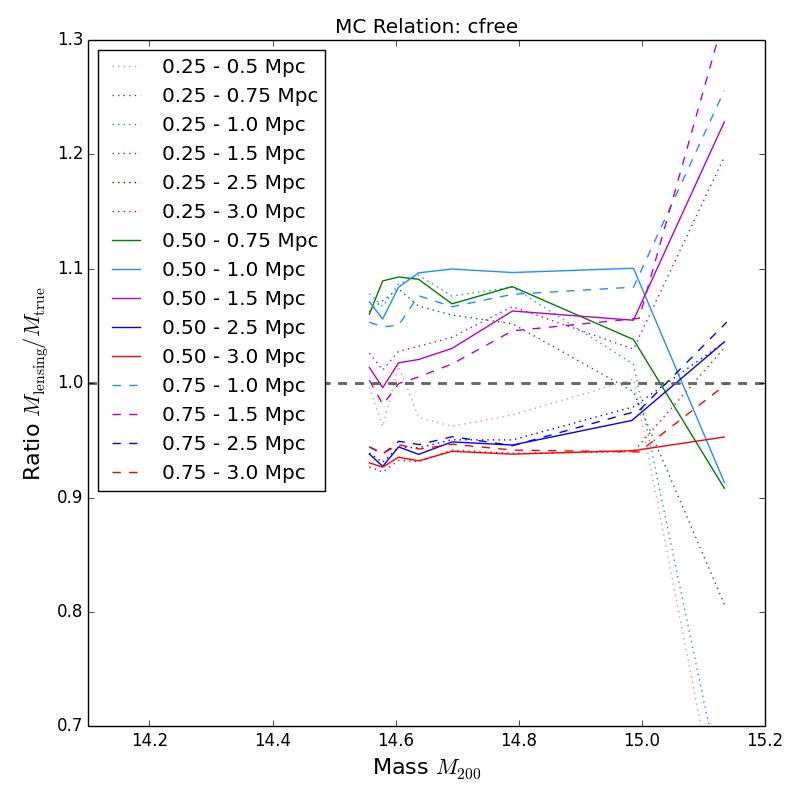
\includegraphics[height=0.65\textheight]{../figures/cfree}\\

{\small MXXL, c-free. Line styles = inner boundary. Color = outer boundary. }

\end{frame}

%%%%%%%%%%%%%%%%%%%%%%%%%%%%%%%%%%%%%%%

\begin{frame}
\frametitle{Profile Uncertainty beyond $R_{vir}$}

\centering

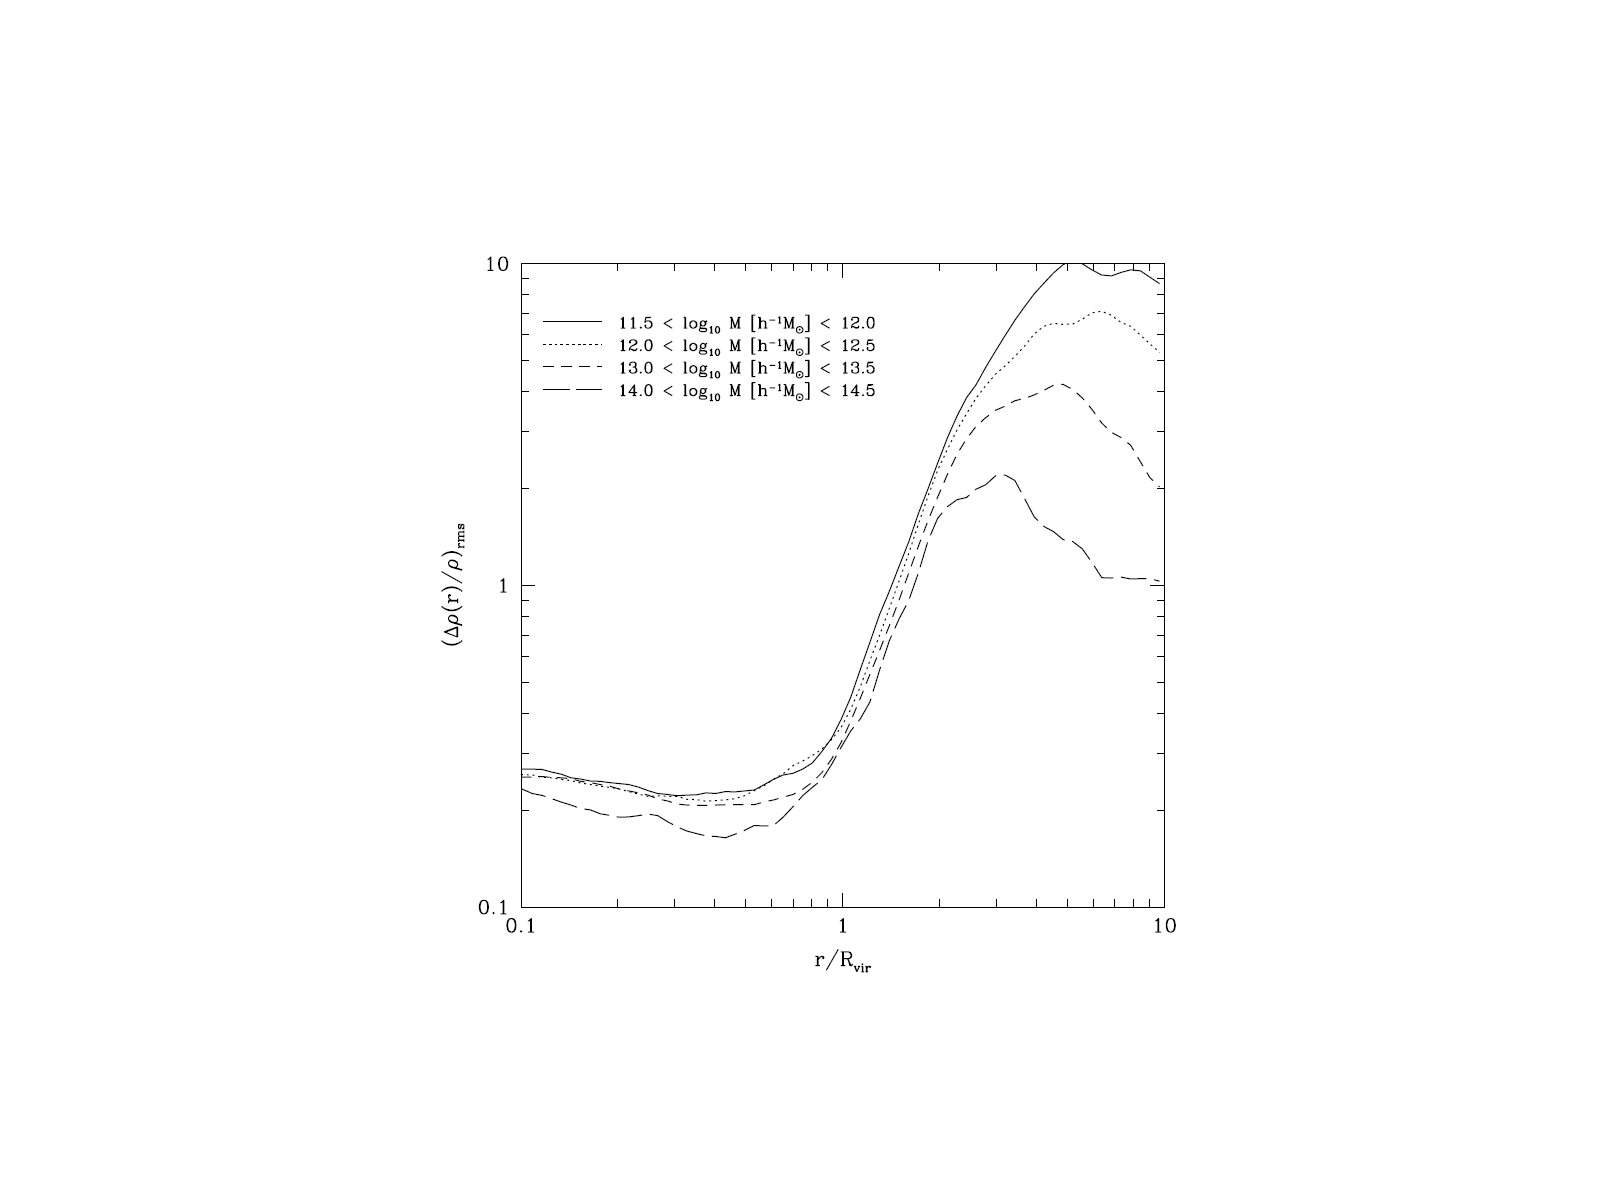
\includegraphics[height=0.85\textheight]{tavio_profile_uncertainty}\\
\tiny{Halo-to-Halo rms scatter in 3D density profile. From Tavio et al.\ 2008.}

\end{frame}

%%%%%%%%%%%%%%%%%%%%%%%%%%%%%%%%%%%%%%%

\begin{frame}
\frametitle{Which mass to calibrate?}

\begin{itemize}
\item Bias depends on $\Delta = {500, 200}$ (BK11)
\item Shouldn't we calibrate $M_{\Delta}$ used in mass-function?
\end{itemize}

\end{frame}

%%%%%%%%%%%%%%%%%%%%%%%%%%%%%%%%%%%%%%%%
%%%%%%%%%%%%%%%%%%%%%%%%%%%%%%%%%%%%%%%%

\begin{frame}
\frametitle{Questions \& Next Steps}

\begin{itemize}
\item Why is the C-free bias different for BK11?
\item Do cosmology-dependent M-C relations work?
\item Are we seeing noise bias?
\item Is the intrinsic noise difference a box vs light-cone issue?
\item Does MXXL also see redshift evolution?
\item Can we eliminate the fit-radius dependence?
\end{itemize}

\end{frame}



\end{document}
